\documentclass[]{standalone}

\begin{document}
	\begin{frame}{Features Extraction}{}
	
	
		\begin{columns}
			\begin{column}{0.45\textwidth}
			\small
			Seven different features were extracted for each segmented lesion:
				\begin{itemize}
				\item Lesion probability;
				\item Label's volume;
				\item Overlapping with boundary region mask;
				\item Overlapping with exclusion region mask;
				\item Probability to belong to each tissue.
				\end{itemize}
			\end{column}
			\begin{column}{0.60\textwidth}
			
			\begin{alertblock}{}
				The boundary and exclusion masks manually segmented on the MNI 152 atlas by expert clinicians.
			\end{alertblock}
			
			\hspace{-10pt}
			\begin{figure}[h!]
			\centering
			\vspace{-20pt}

				\begin{subfigure}{0.4\textwidth}
					\centering
					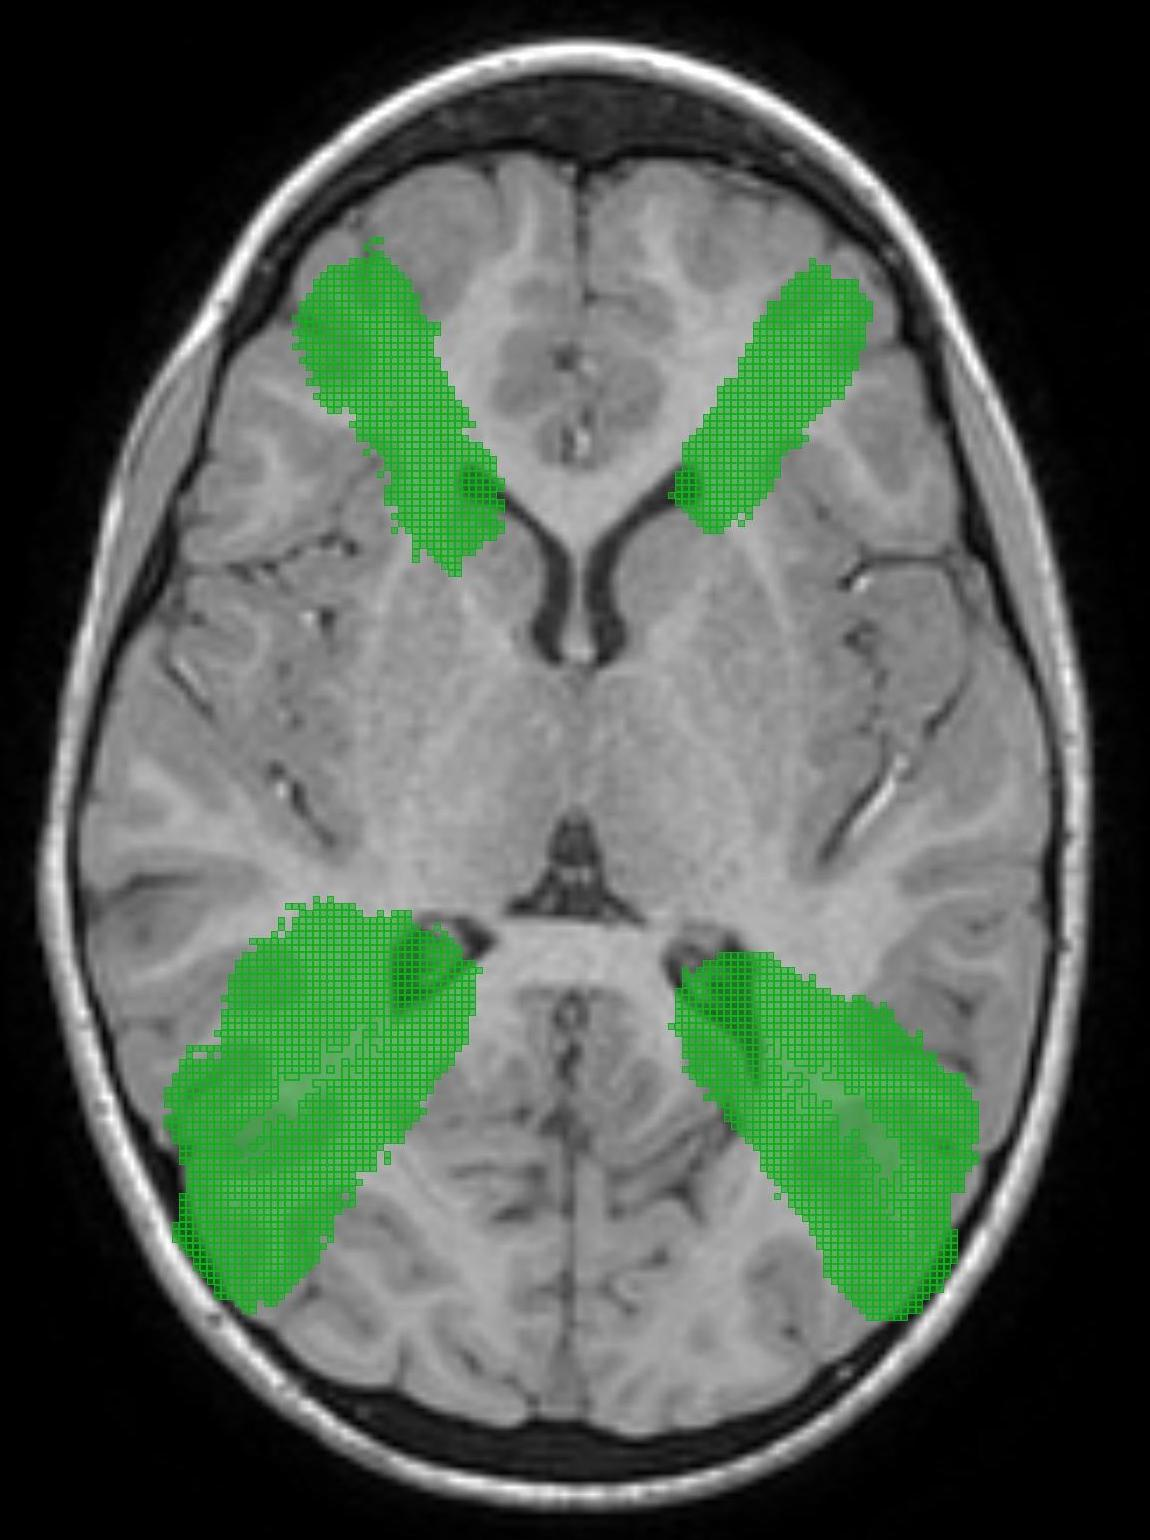
\includegraphics[scale=0.07]{./IMG/boundary.jpg}
					\caption*{Boundary.}
				\end{subfigure}
				\hspace{15pt}
				\begin{subfigure}{0.4\textwidth}
					\centering
					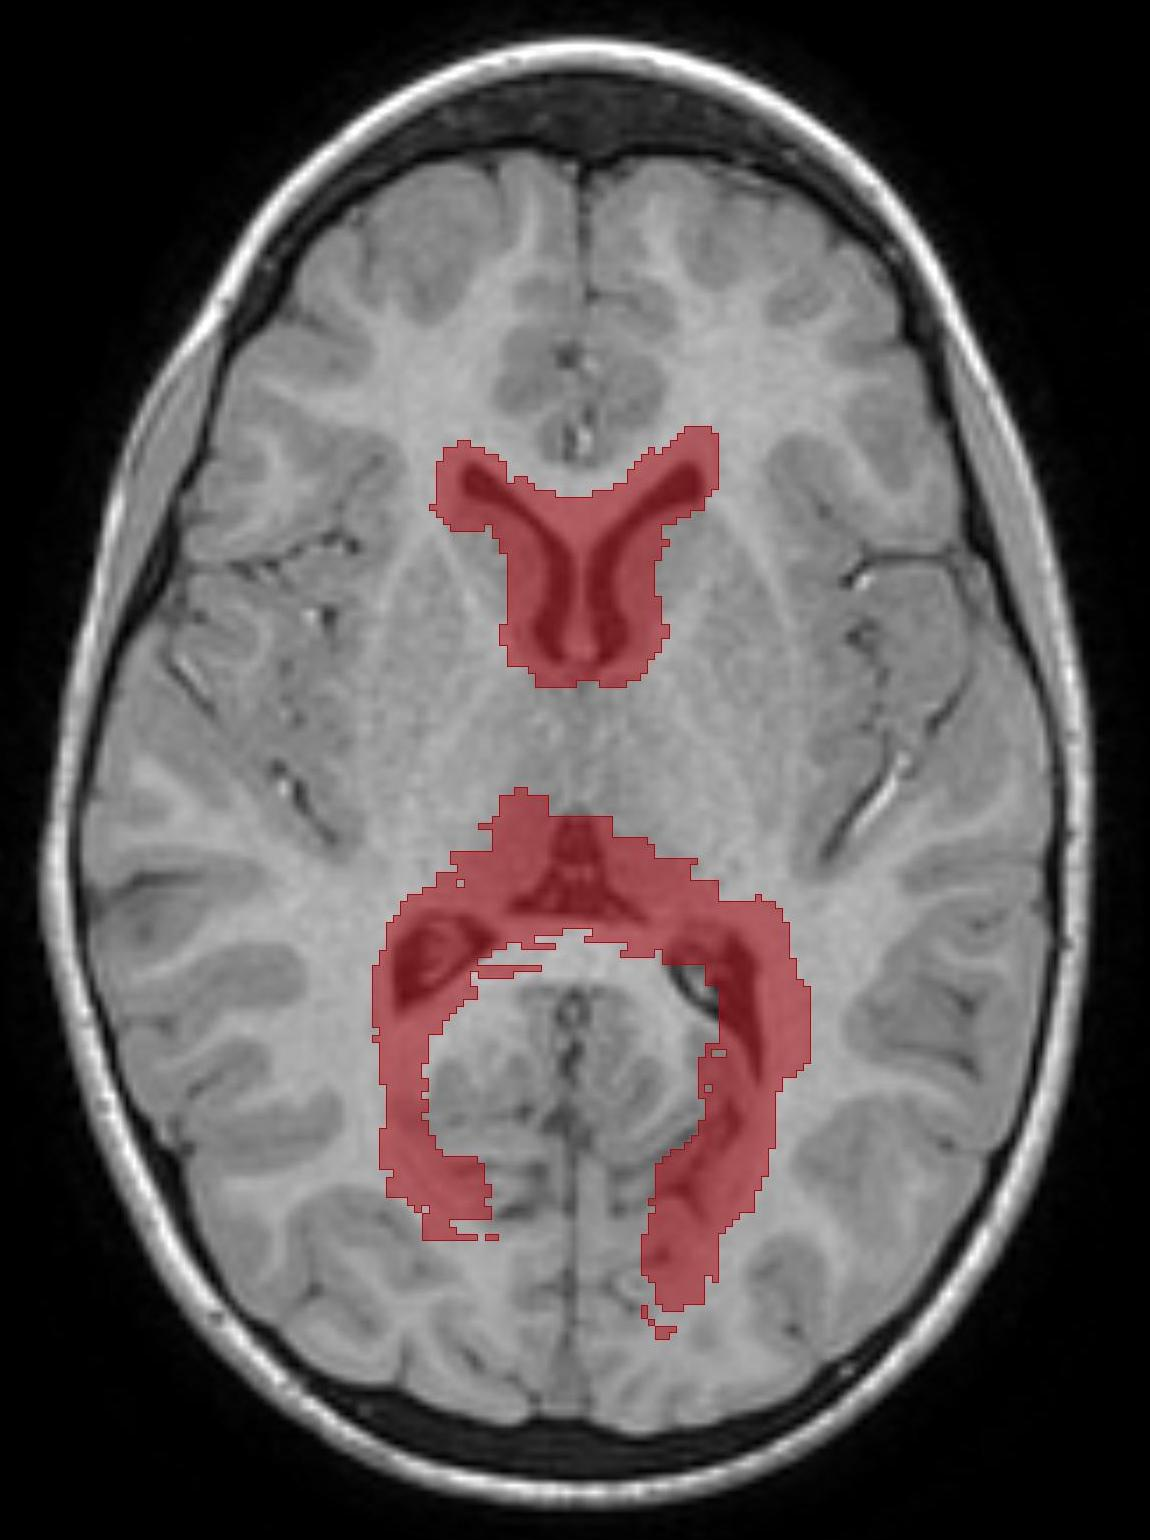
\includegraphics[scale=0.07]{./IMG/exclude.jpg}
					\caption*{Exclusion.}
				\end{subfigure}
			\end{figure}
			\end{column}
		\end{columns}
	\end{frame}
\end{document}
